\documentclass{article}
\usepackage[T1]{fontenc}

\usepackage[utf8]{inputenc}
\usepackage[english]{babel}
\usepackage{upgreek}
\usepackage{amsmath}
\usepackage{color}
\usepackage{listings}
\usepackage{graphicx}

\begin{document}
  \title{Hw05 - Report - Distributed Systems}
  \date{}
  \author{Lukas Dötlinger, 01518316}
	
  \maketitle
  
  \section*{Introduction}
  
  	Both parts of the homework sheet are completed.\\
  	The theoretical exercises of this homework can be found in the next section. The practical program is located in the \texttt{practical/} directory.\\
  	
  \section*{Part 1)}
  
    \subsection*{a)}
    
      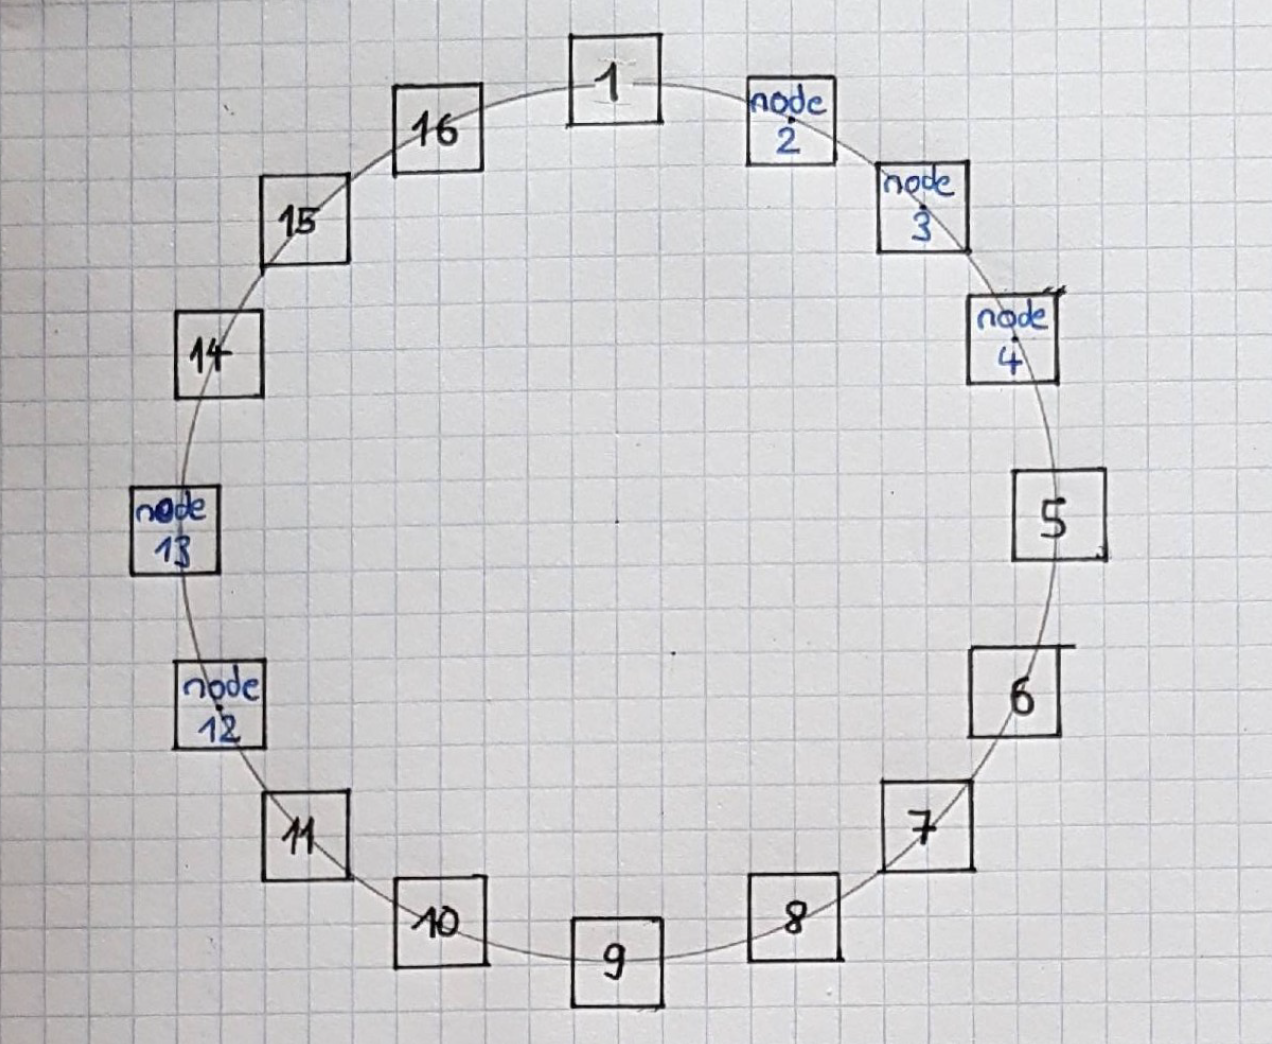
\includegraphics[width=12cm]{chord-drawing.png} \\
      
      Nodes are placed according to my matricular number 1518316 and the given algorithm, which is also implemented as a function, \texttt{getNodePositions(String matrNumber)}, and can be found in \texttt{practical/Utils.java}.\\
      
    \subsection*{b)}
    
      \begin{tabular}{ |l|c|c| } 
      	\hline
      	\multicolumn{3}{|c|}{Node 2} \\
      	\hline
      	Formula & Result & Successor \\
      	\hline
      	$(2+2^0)\%16$ & 3 & 3 \\ 
      	$(2+2^1)\%16$ & 4 & 4 \\ 
      	$(2+2^2)\%16$ & 6 & 12 \\ 
      	$(2+2^3)\%16$ & 10 & 12 \\
      	\hline
      \end{tabular}
      \quad
  	  \begin{tabular}{ |l|c|c| } 
  	  	\hline
  	  	\multicolumn{3}{|c|}{Node 3} \\
  	  	\hline
  	  	Formula & Result & Successor \\
  	  	\hline
  	  	$(3+2^0)\%16$ & 4 & 4 \\ 
  	  	$(3+2^1)\%16$ & 5 & 12 \\ 
  	  	$(3+2^2)\%16$ & 7 & 12 \\ 
  	  	$(3+2^3)\%16$ & 11 & 12 \\
  	  	\hline
  	  \end{tabular} \\
      \quad
      \begin{tabular}{ |l|c|c| } 
      	\hline
      	\multicolumn{3}{|c|}{Node 4} \\
      	\hline
      	Formula & Result & Successor \\
      	\hline
      	$(4+2^0)\%16$ & 5 & 12 \\ 
      	$(4+2^1)\%16$ & 6 & 12 \\ 
      	$(4+2^2)\%16$ & 8 & 12 \\ 
      	$(4+2^3)\%16$ & 12 & 12 \\
      	\hline
      \end{tabular}
      \quad
      \begin{tabular}{ |l|c|c| } 
      	\hline
      	\multicolumn{3}{|c|}{Node 12} \\
      	\hline
      	Formula & Result & Successor \\
      	\hline
      	$(12+2^0)\%16$ & 13 & 13 \\ 
      	$(12+2^1)\%16$ & 14 & 2 \\ 
      	$(12+2^2)\%16$ & 16 & 2 \\ 
      	$(12+2^3)\%16$ & 4 & 4 \\
      	\hline
      \end{tabular}\\
      \quad
      \begin{tabular}{ |l|c|c| } 
      	\hline
      	\multicolumn{3}{|c|}{Node 13} \\
      	\hline
      	Formula & Result & Successor \\
      	\hline
      	$(13+2^0)\%16$ & 14 & 2 \\ 
      	$(13+2^1)\%16$ & 15 & 2 \\ 
      	$(13+2^2)\%16$ & 1 & 2 \\ 
      	$(13+2^3)\%16$ & 5 & 12 \\
      	\hline
      \end{tabular}\\
  
    \subsection*{c)}
    
      Node MIN to Node MAX -> \textbf{Node 2 to Node 13}. \\
      \newline
      \begin{tabular}{ |c| } 
      	\hline
      	\textbf{iterative} \\
      	Steps \\
      	\hline
      	Node 2 passes the query to Node 3\\
      	Node 2 passes the query to Node 4\\
      	Node 2 passes the query to Node 12\\
      	Node 12's immediate successor is Node 13\\
      	\hline
      \end{tabular}
      \quad
      \begin{tabular}{ |c| } 
      	\hline
      	\textbf{recursive} \\
      	Steps \\
      	\hline
      	Node 2 passes the query to Node 12\\
      	Node 12's immediate successor is Node 13\\
      	\hline
      \end{tabular}\\
  
    \newpage
    \subsection*{d)}
    
      Node MAX to Node MIN -> \textbf{Node 13 to Node 2}. \\
      \newline
      \begin{tabular}{ |c| } 
      	\hline
      	\textbf{iterative} \\
      	Steps \\
      	\hline
      	Node 13 passes the query to Node 2\\
      	Node 2 is the required Node\\
      	\hline
      \end{tabular}
      \quad
      \begin{tabular}{ |c| } 
      	\hline
      	\textbf{recursive} \\
      	Steps \\
      	\hline
      	Node 13 passes the query to Node 12\\
      	Node 13 passes the query to Node 2\\
      	Node 2 is the required Node\\
      	\hline
      \end{tabular}\\  
  
  \section*{Part 2)}
  
    Part 2 is implemented in Java-Code. The code can be found in the \texttt{practical/} directory. It simulates a chord using a list of \texttt{Node} objects. Each node computes its own finger-table and reacts to another node leaving or joining by updating it's table, successor and predecessor fields. The \texttt{Main.java} controls and starts everything. After a change, for example a node joining, all nodes update itself. Every-time something changes, the fields of a node get printed.\\
    \newline
    To run the code, simply execute the java class \texttt{Main.java}, which is located in the \texttt{practical/} directory.\\
    \newline
    The output of a node being printed looks like this:\\
    \newline
    \begin{lstlisting}[language=sh]
      -----node2-----
      Successor | Id: 3 | Name: node3 | Address: localhost:8003
      Predecessor | Id: 12 | Name: node12 | Address: localhost:80012
      Id: 3 | Name: node3 | Address: localhost:8003
      Id: 4 | Name: node4 | Address: localhost:8004
      Id: 7 | Name: node7 | Address: localhost:8007
      Id: 12 | Name: node12 | Address: localhost:80012
      ---------------
    \end{lstlisting}
  
\end{document}